\documentclass[11pt,a4paper]{article}
\usepackage{graphicx,fancyhdr,natbib,subfigure}
\usepackage{epsfig, epsf}
\usepackage{amsmath, cancel, amssymb}
\usepackage{lscape, longtable, caption}
\usepackage{multirow}
\usepackage{dcolumn}% Align table columns on decimal point
\usepackage{bm}% bold math
\usepackage{hyperref,ifthen}
\usepackage{verbatim}
\usepackage{color}
\usepackage[usenames,dvipsnames]{xcolor}
%% http://en.wikibooks.org/wiki/LaTeX/Colors



%%%%%%%%%%%%%%%%%%%%%%%%%%%%%%%%%%%%%%%%%%%
%       define Journal abbreviations      %
%%%%%%%%%%%%%%%%%%%%%%%%%%%%%%%%%%%%%%%%%%%
\def\nat{Nat} \def\apjl{ApJ~Lett.} \def\apj{ApJ}
\def\apjs{ApJS} \def\aj{AJ} \def\mnras{MNRAS}
\def\prd{Phys.~Rev.~D} \def\prl{Phys.~Rev.~Lett.}
\def\plb{Phys.~Lett.~B} \def\jhep{JHEP} \def\nar{NewAR}
\def\npbps{NUC.~Phys.~B~Proc.~Suppl.} \def\prep{Phys.~Rep.}
\def\pasp{PASP} \def\aap{Astron.~\&~Astrophys.} \def\araa{ARA\&A}
\def\pasa{PASA}
\def\jcap{\ref@jnl{J. Cosmology Astropart. Phys.}}%
\def\physrep{Phys.~Rep.}


\newcommand{\preep}[1]{{\tt #1} }

%%%%%%%%%%%%%%%%%%%%%%%%%%%%%%%%%%%%%%%%%%%%%%%%%%%%%
%              define symbols                       %
%%%%%%%%%%%%%%%%%%%%%%%%%%%%%%%%%%%%%%%%%%%%%%%%%%%%%
\def \Mpc {~{\rm Mpc} }
\def \Om {\Omega_0}
\def \Omb {\Omega_{\rm b}}
\def \Omcdm {\Omega_{\rm CDM}}
\def \Omlam {\Omega_{\Lambda}}
\def \Omm {\Omega_{\rm m}}
\def \ho {H_0}
\def \qo {q_0}
\def \lo {\lambda_0}
\def \kms {{\rm ~km~s}^{-1}}
\def \kmsmpc {{\rm ~km~s}^{-1}~{\rm Mpc}^{-1}}
\def \hmpc{~\;h^{-1}~{\rm Mpc}} 
\def \hkpc{\;h^{-1}{\rm kpc}} 
\def \hmpcb{h^{-1}{\rm Mpc}}
\def \dif {{\rm d}}
\def \mlim {m_{\rm l}}
\def \bj {b_{\rm J}}
\def \mb {M_{\rm b_{\rm J}}}
\def \mg {M_{\rm g}}
\def \qso {_{\rm QSO}}
\def \lrg {_{\rm LRG}}
\def \gal {_{\rm gal}}
\def \xibar {\bar{\xi}}
\def \xis{\xi(s)}
\def \xisp{\xi(\sigma, \pi)}
\def \Xisig{\Xi(\sigma)}
\def \xir{\xi(r)}
\def \max {_{\rm max}}
\def \gsim { \lower .75ex \hbox{$\sim$} \llap{\raise .27ex \hbox{$>$}} }
\def \lsim { \lower .75ex \hbox{$\sim$} \llap{\raise .27ex \hbox{$<$}} }
\def \deg {^{\circ}}
%\def \sqdeg {\rm deg^{-2}}
\def \deltac {\delta_{\rm c}}
\def \mmin {M_{\rm min}}
\def \mbh  {M_{\rm BH}}
\def \mdh  {M_{\rm DH}}
\def \msun {M_{\odot}}
\def \z {_{\rm z}}
\def \edd {_{\rm Edd}}
\def \lin {_{\rm lin}}
\def \nonlin {_{\rm non-lin}}
\def \wrms {\langle w_{\rm z}^2\rangle^{1/2}}
\def \dc {\delta_{\rm c}}
\def \wp {w_{p}(\sigma)}
\def \PwrSp {\mathcal{P}(k)}
\def \DelSq {$\Delta^{2}(k)$}
\def \WMAP {{\it WMAP \,}}
\def \cobe {{\it COBE }}
\def \COBE {{\it COBE \;}}
\def \HST  {{\it HST \,\,}}
\def \Spitzer  {{\it Spitzer \,}}
\def \ATLAS {VST-AA$\Omega$ {\it ATLAS} }
\def \BEST   {{\tt best} }
\def \TARGET {{\tt target} }
\def \TQSO   {{\tt TARGET\_QSO}}
\def \HIZ    {{\tt TARGET\_HIZ}}
\def \FIRST  {{\tt TARGET\_FIRST}}
\def \zc {z_{\rm c}}
\def \zcz {z_{\rm c,0}}

\newcommand{\ltsim}{\raisebox{-0.6ex}{$\,\stackrel
        {\raisebox{-.2ex}{$\textstyle <$}}{\sim}\,$}}
\newcommand{\gtsim}{\raisebox{-0.6ex}{$\,\stackrel
        {\raisebox{-.2ex}{$\textstyle >$}}{\sim}\,$}}
\newcommand{\simlt}{\raisebox{-0.6ex}{$\,\stackrel
        {\raisebox{-.2ex}{$\textstyle <$}}{\sim}\,$}}
\newcommand{\simgt}{\raisebox{-0.6ex}{$\,\stackrel
        {\raisebox{-.2ex}{$\textstyle >$}}{\sim}\,$}}

\newcommand{\Msun}{M_\odot}
\newcommand{\Lsun}{L_\odot}
\newcommand{\lsun}{L_\odot}
\newcommand{\Mdot}{\dot M}

\newcommand{\sqdeg}{deg$^{-2}$}
\newcommand{\hi}{H\,{\sc i}\ }
\newcommand{\lya}{Ly$\alpha$\ }
%\newcommand{\lya}{Ly\,$\alpha$\ }
\newcommand{\lyaf}{Ly\,$\alpha$\ forest}
%\newcommand{\eg}{e.g.~}
%\newcommand{\etal}{et~al.~}
\newcommand{\lyb}{Ly$\beta$\ }
\newcommand{\cii}{C\,{\sc ii}\ }
\newcommand{\ciii}{C\,{\sc iii}]\ }
\newcommand{\civ}{C\,{\sc iv}\ }
\newcommand{\SiII}{Si\,{\sc ii}\ }
\newcommand{\SiIV}{Si\,{\sc iv}\ }
\newcommand{\mgii}{Mg\,{\sc ii}\ }
\newcommand{\feii}{Fe\,{\sc ii}\ }
\newcommand{\feiii}{Fe\,{\sc iii}\ }
\newcommand{\caii}{Ca\,{\sc ii}\ }
\newcommand{\halpha}{H\,$\alpha$\ }
\newcommand{\hbeta}{H\,$\beta$\ }
\newcommand{\hgamma}{H\,$\gamma$\ }
\newcommand{\hdelta}{H\,$\delta$\ }
\newcommand{\oi}{[O\,{\sc i}]\ }
\newcommand{\oii}{[O\,{\sc ii}]\ }
\newcommand{\oiii}{[O\,{\sc iii}]\ }
\newcommand{\heii}{He\,{\sc ii}\ }
%\newcommand{\heii}{[He\,{\sc ii}]\ }
\newcommand{\nv}{N\,{\sc v}\ }
\newcommand{\nev}{Ne\,{\sc v}\ }
\newcommand{\neiii}{[Ne\,{\sc iii}]\ }
\newcommand{\alii}{Al\,{\sc ii}\ }
\newcommand{\aliii}{Al\,{\sc iii}\ }
\newcommand{\siiii}{Si\,{\sc iii}]\ }


\begin{document}

   \title{Colour-colour plots for VH$z$Q Selection}
 \date{\today}
\maketitle

\section{(z-J) vs. (J-W1)}
    \begin{figure}
      \centering
      % trim={<left> <lower> <right> <upper>}
      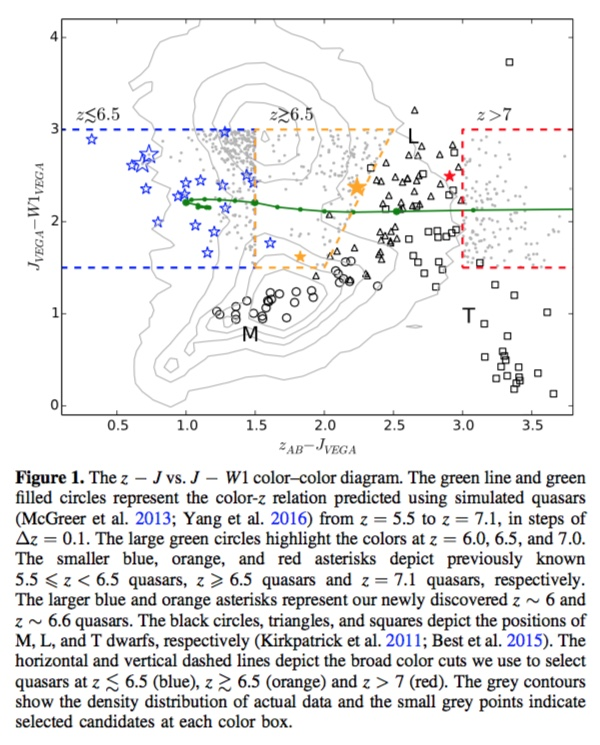
\includegraphics[width=16.0cm, trim={0.5cm 0 0 0},clip]
      {Wang2017_Fig1.jpeg}
      \caption[]{\citet{Wang2017}}
      \label{fig:Wang2017}
    \end{figure}


\section{(z-y) vs. (y-J)}

    \begin{figure}
      \begin{center}
      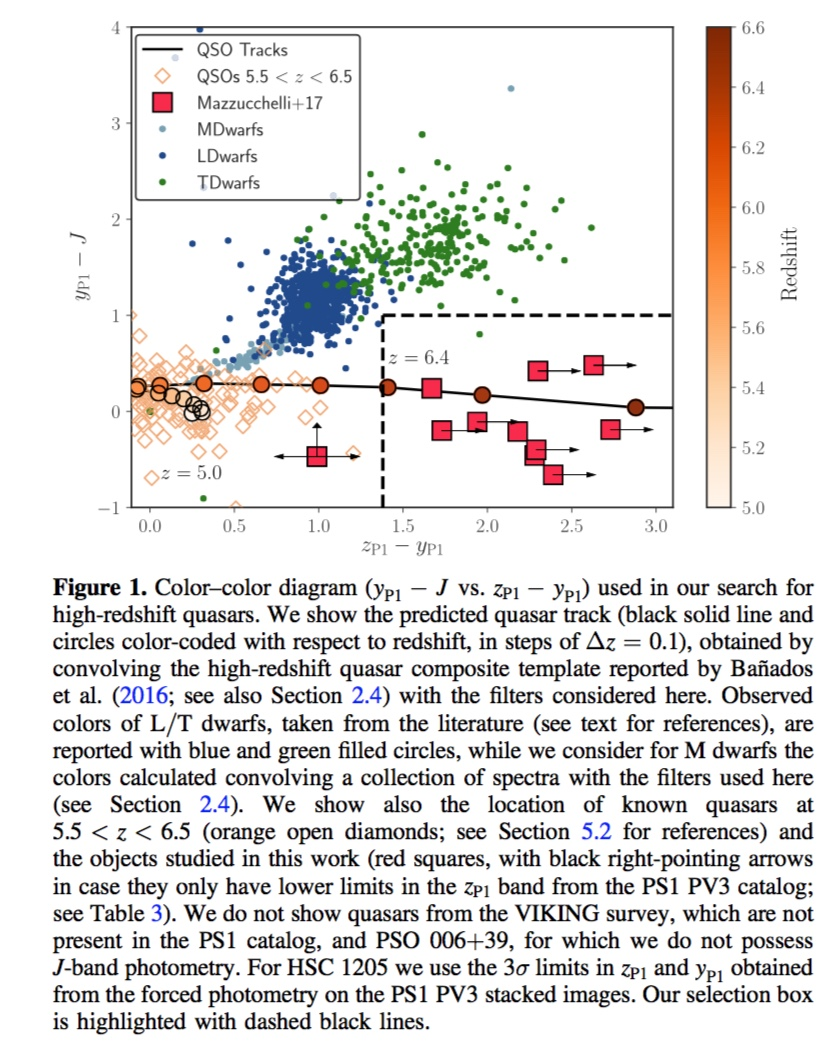
\includegraphics[width=16.0cm,  trim={1.5cm 0 0 0},clip]
      {Mazzucchelli_2017_Fig1.jpeg}
     \caption[]{\citet{Mazzucchelli2017}}
      \label{fig:Mazzucchelli2017}
      \end{center}
    \end{figure}


\section{(i-z) vs. (z-y)}
    \begin{figure}
      \centering
      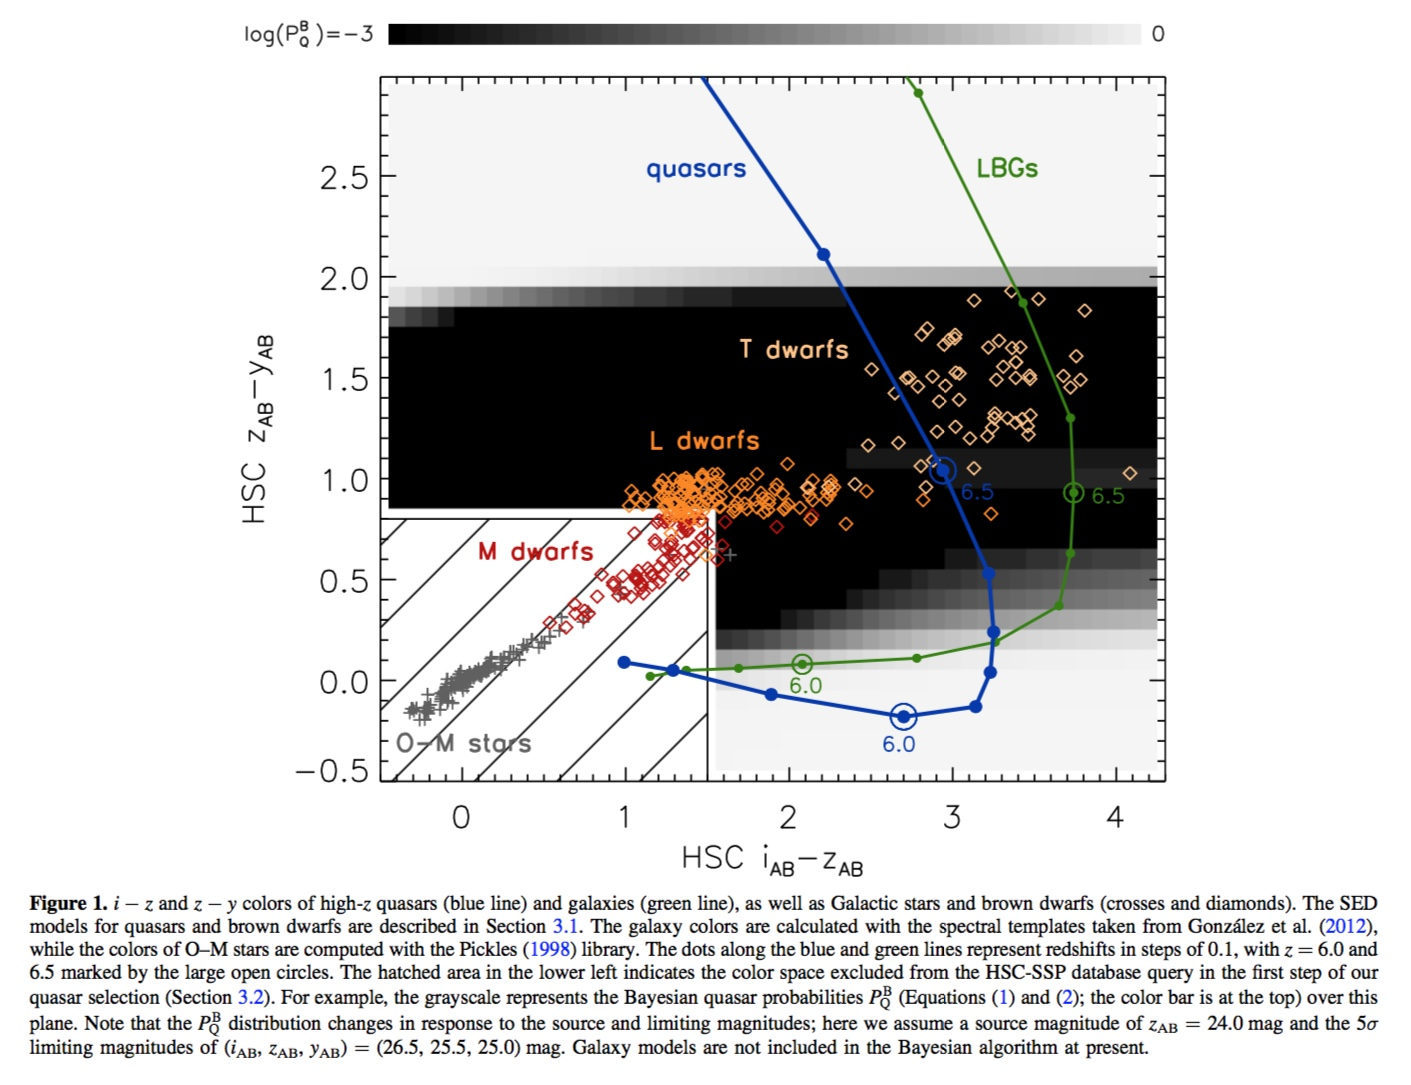
\includegraphics[width=16.0cm,  trim={1.5cm 0 0 0},clip]
      {Matsuoka_2016_Fig1.jpeg}
      \caption[]{\citet{Matsuoka2016}}
      \label{fig:Matsuoka2016}
    \end{figure}

    \begin{figure}
      \centering
      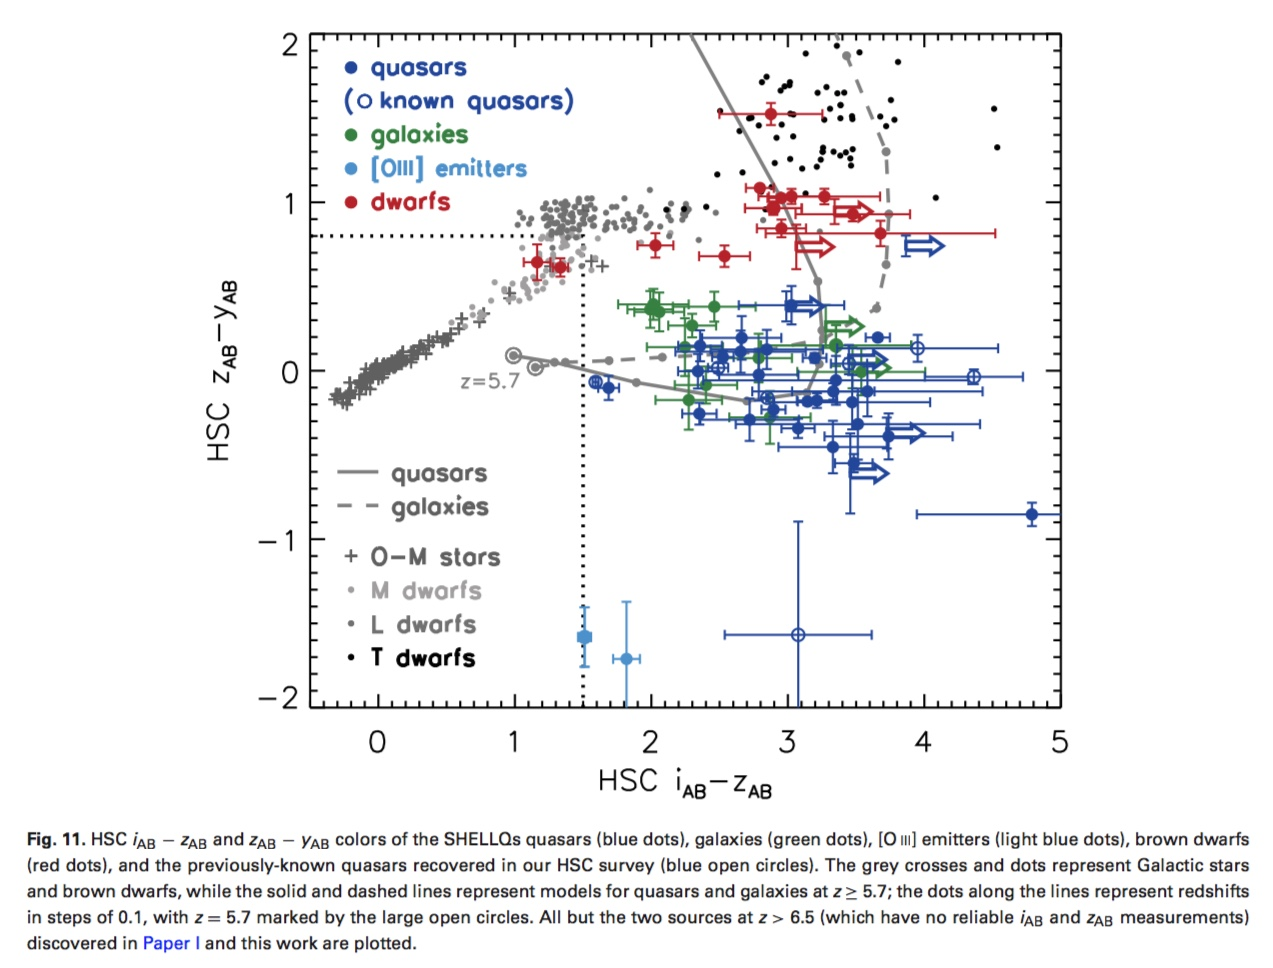
\includegraphics[width=16.0cm,  trim={1.5cm 0 0 0},clip]
      {Matsuoka_2018_Fig11.jpeg}
      \caption[]{\citet{Matsuoka2018}}
      \label{fig:Matsuoka2018}
    \end{figure}


\section{(z-y) vs. (i-z)}

    \begin{figure}
      \centering
%      \includegraphics[width=16.0cm,  trim={1.5cm 0 0 0},clip, angle=90]
      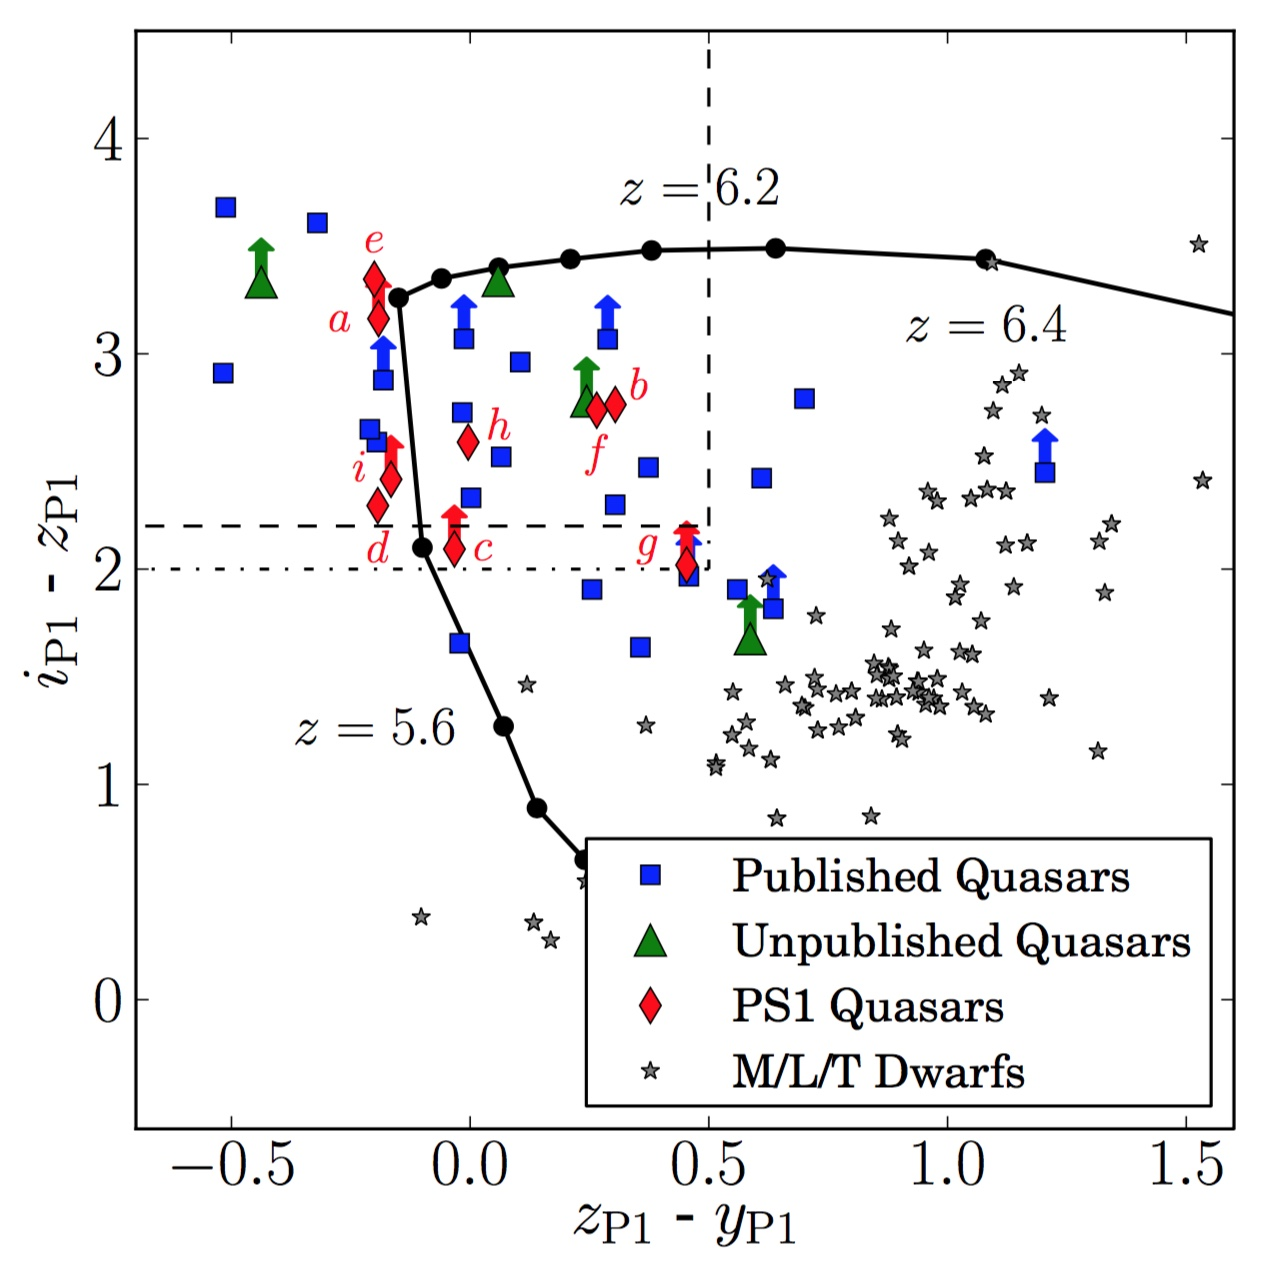
\includegraphics[width=16.0cm,  trim={0.0cm 0 0 0},clip, angle=0]
      {Banados_2014_Fig1.jpeg}
      \caption[]{\citet{Banados2014}. 
        Right: color–color diagram showing the criteria used to select quasar
        candidates (long-dashed line, upper left corner). The dot-dashed line
        is used for candidates with upper limits in the iP1 band. The thick
        black line shows the expected color of the quasar template from
        \citet{Decarli2010} redshifted from $z=5.0$ to $z=6.5$ in steps of
        $\Delta z = 0.1$ (see left panel). The M/L/T dwarfs from \citet{Dupuy_Liu2012}  that have a PS1 counterpart are shown with stars. Blue squares are
        published quasars at 5.7 < z < 6.4 satisfying our S/N and coverage
        criteria. Fourteen of them were included in our candidate list. Green
        triangles represent the PS1 colors of unpublished spectroscopically
        confirmed z ∼ 6 quasars (S. J. Warren et al., in preparation). Three
        of them were part of our candidate list (see Tables 4 and 5). The red
        diamonds are the new quasars presented in this paper (see Table
        2). They are labeled with the following letters: a = PSO
        J340.2041–18.6621 (z = 6.00), b = PSO J007.0273+04.9571 (z = 5.99), c
        = PSO J037.9706–28.8389 (z = 5.99), d = PSO J187.3050+04.3243 (z =
        5.89), e = PSO J213.3629–22.5617 (z = 5.88), f = PSO J183.2991–12.7676
        (z = 5.86), g = PSO J210.8722–12.0094 (z = 5.84), h = PSO
        J215.1514–16.0417 (z = 5.73), and i = PSO J045.1840–22.5408 (z =
        5.70).
}
      \label{fig:Banados2014}
    \end{figure}

    \begin{figure}
      \centering
%      \includegraphics[width=16.0cm,  trim={1.5cm 0 0 0},clip, angle=90]
      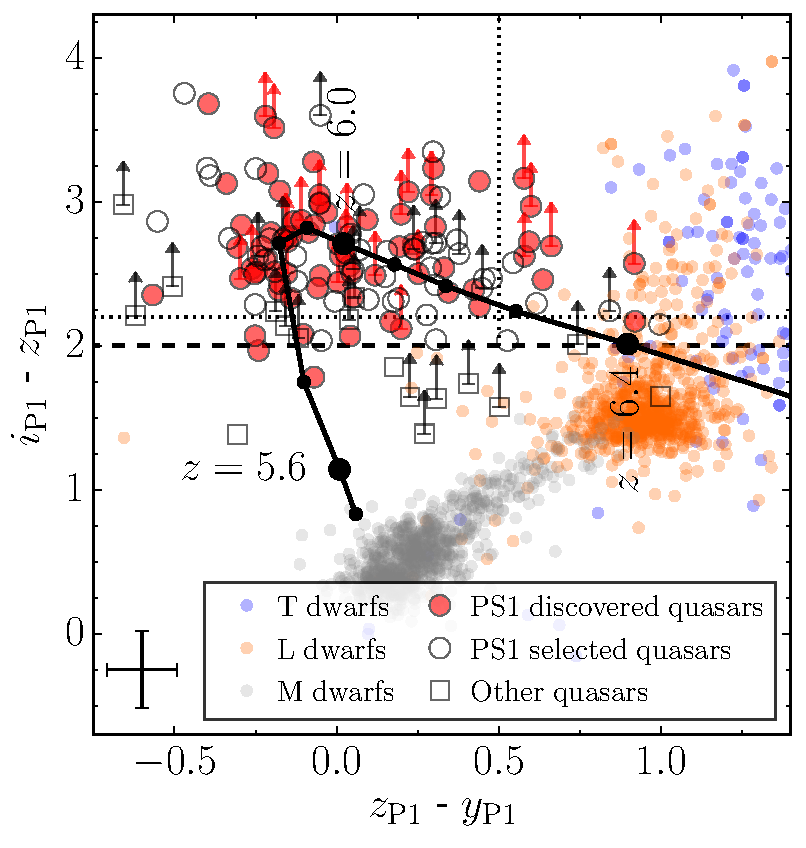
\includegraphics[width=16.0cm,  trim={0.0cm 0 0 0},clip, angle=0]{f1_ps1_color_selection.pdf}
      \caption[]{\citet{Banados2016}.} 
      \label{fig:Banados2016}
    \end{figure}


\section{(W1 - W2) vs. (z - W2)}
    \begin{figure}
      \centering
      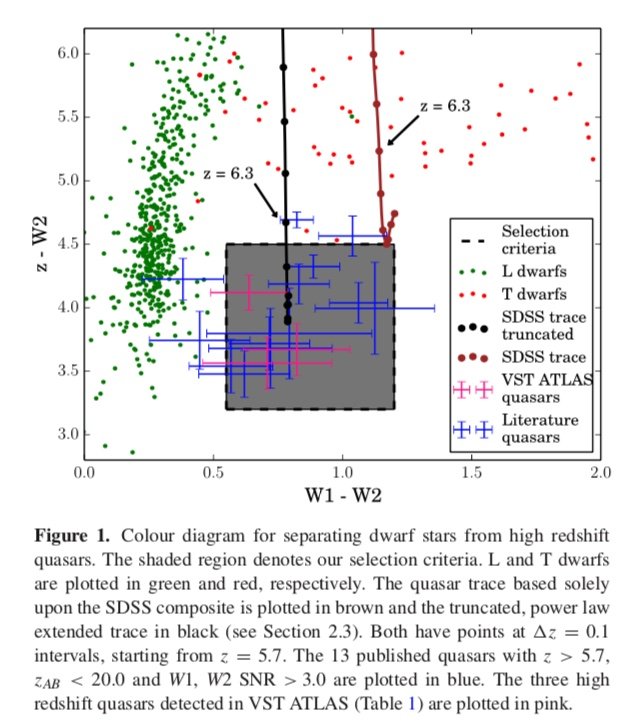
\includegraphics[width=16.0cm,  trim={0.0cm 0 0 0},clip, angle=0]{Carnall_2015_Fig1.jpeg}
      \caption[]{\citet{Banados2016}.} 
      \label{fig:Banados2016}
    \end{figure}


\newpage
    \begin{figure}
      \centering
      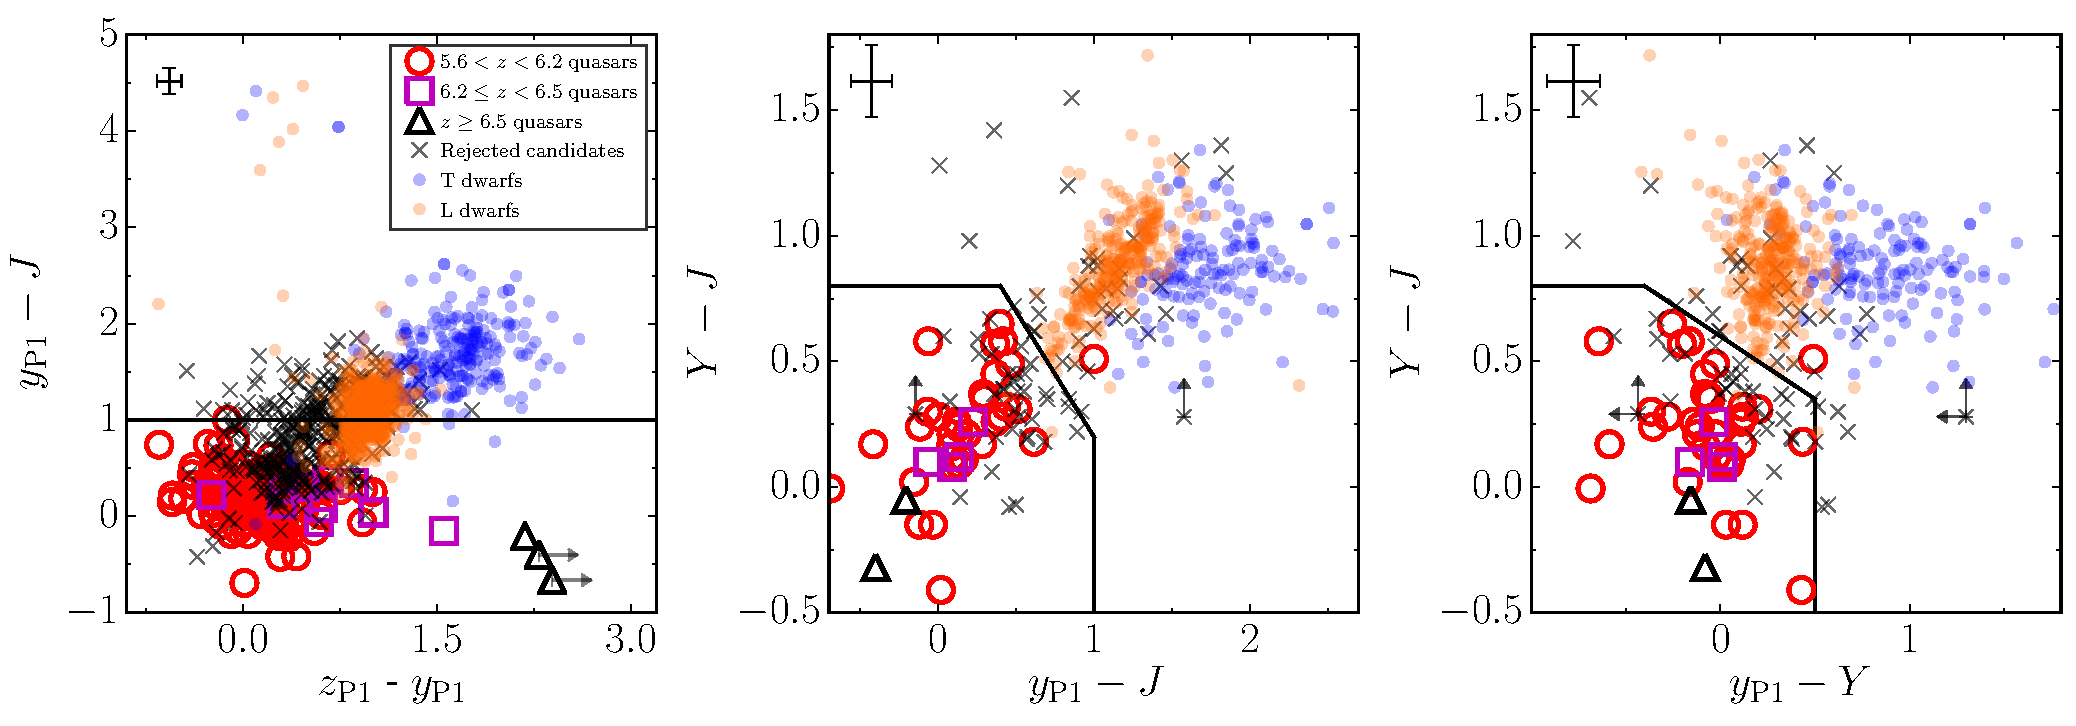
\includegraphics[width=16.0cm,  trim={0.0cm 0 0 0},clip, angle=0]{f4_yj_selection.pdf}
      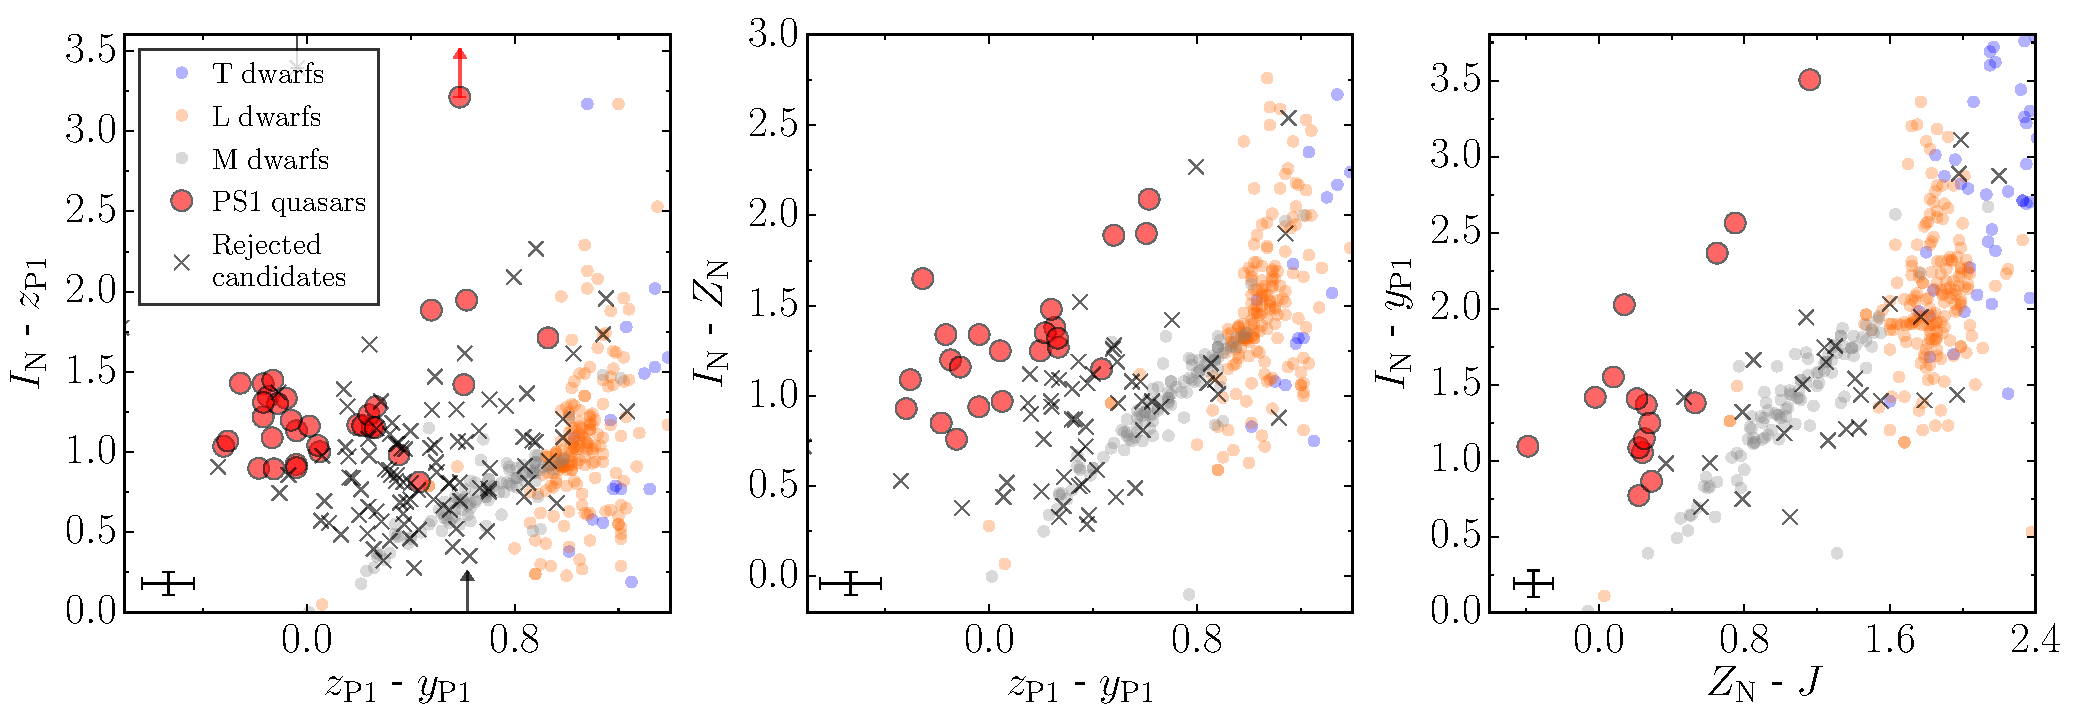
\includegraphics[width=16.0cm,  trim={0.0cm 0 0 0},clip, angle=0]{f6_ntt_colors.pdf}
      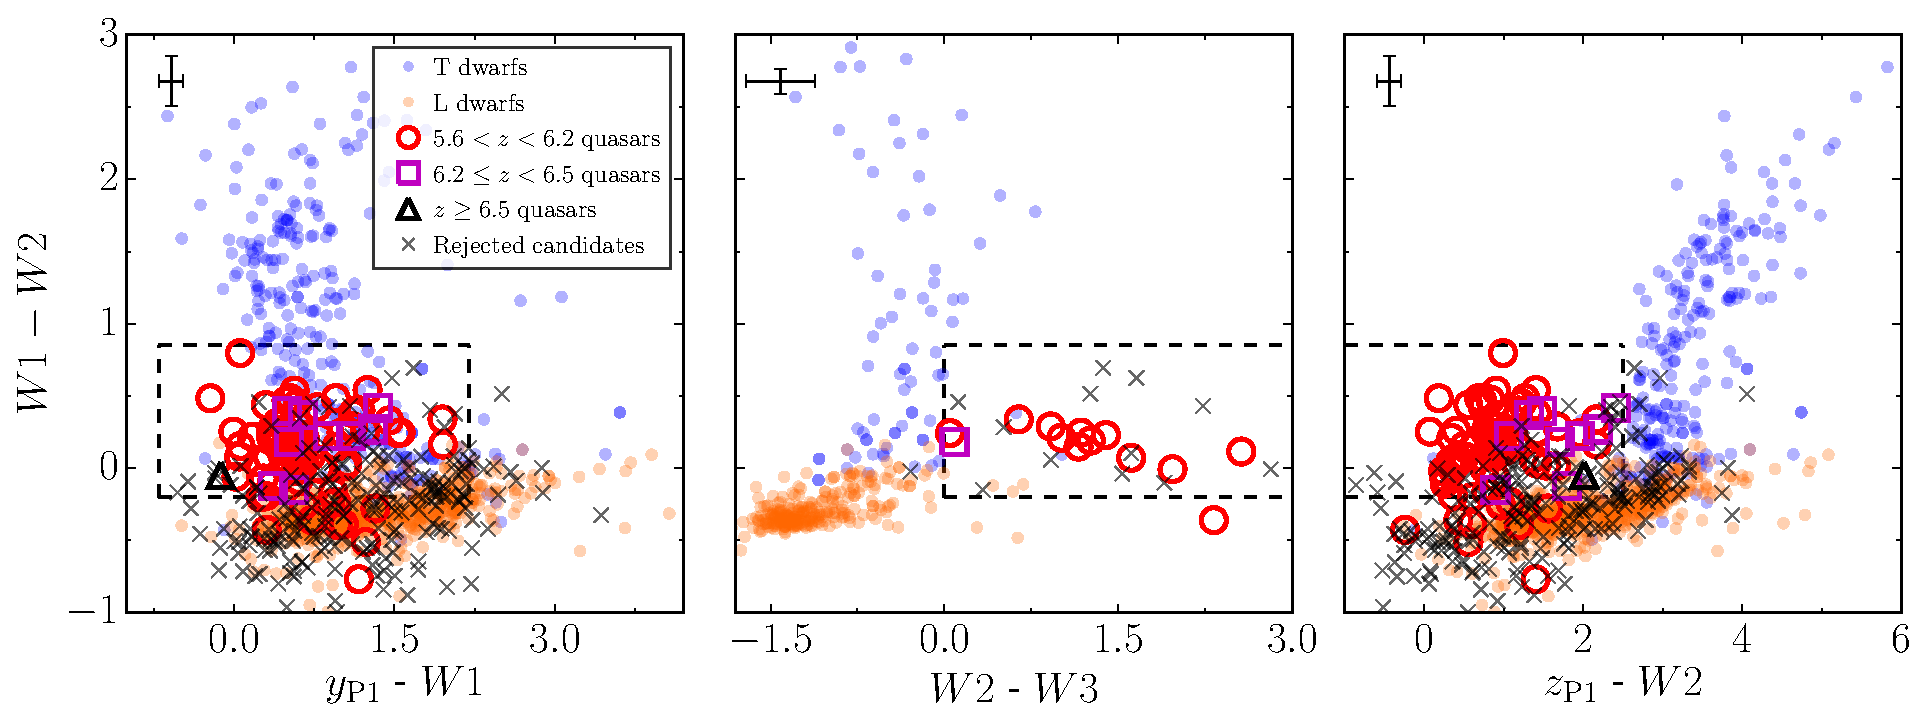
\includegraphics[width=16.0cm,  trim={0.0cm 0 0 0},clip, angle=0]{f5_wise_prioritization.pdf}
      \caption[]{\citet{Banados2016}.} 
      \label{fig:Banados2016_3panels}
    \end{figure}





\bibliographystyle{mn2e}
\bibliography{/cos_pc19a_npr/LaTeX/tester_mnras}


\end{document}